\section{Background}
\label{sec:background}
\subsection{Short introduction to parallel Haskells}
There are already several ways to write parallel programs in Haskell. As we will base our parallel arrows on existing parallel Haskells, we will now give a short introduction to the ones we use as backends in this paper.

In its purest form, parallel computation (on functions) can be looked at as the execution of some functions \code{a -> b} in parallel:

\begin{lstlisting}[frame=htrbl]
parEvalN :: [a -> b] -> [a] -> [b]
\end{lstlisting}
\begin{center}
	\includegraphics[scale=0.7]{images/parEvalN}
\end{center}
Before we go into detail on how we can use this idea of parallelism for parallel Arrows, as a short introduction to parallelism in Haskell we will now implement \code{parEvalN} with several different parallel Haskells.

\subsubsection{Multicore Haskell}
Multicore Haskell \cite{Marlow2009} is way to do parallel processing found in standard GHC.\footnote{See \url{https://hackage.haskell.org/package/parallel-3.2.1.0}.} It ships with parallel evaluation strategies for several types which can be applied with \code{using :: a -> Strategy a -> a}. For \code{parEvalN} this means that we can just apply the list of functions \code{[a -> b]} to the list of inputs \code{[a]} by zipping them with the application operator \code{\$}. We then evaluate this lazy list \code{[b]} according to a \code{Strategy [b]} with the \code{using :: a -> Strategy a -> a} operator. We construct this strategy with \code{parList :: Strategy a -> Strategy [a]} and \code{rdeepseq :: NFData a => Strategy a} where the latter is a strategy which evalutes to normal form. To ensure that programs that use \code{parEvalN} have the correct evaluation order, we annotate the computation with \code{pseq :: a -> b -> b} which forces the compiler to not reorder multiple \code{parEvalN} computations. This is particularly necessary in circular communication topologies like in the \code{torus} or \code{ring} skeleton that we will see in chapter \ref{sec:topology-skeletons} which resulted in deadlock scenarios when executed without \code{pseq} during testing for this paper.

\begin{lstlisting}[frame=htrbl]
parEvalN :: (NFData b) => [a -> b] -> [a] -> [b]
parEvalN fs as = let bs = zipWith ($) fs as in
	(bs `using` parList rdeepseq) `pseq` bs
\end{lstlisting}
\begin{center}
	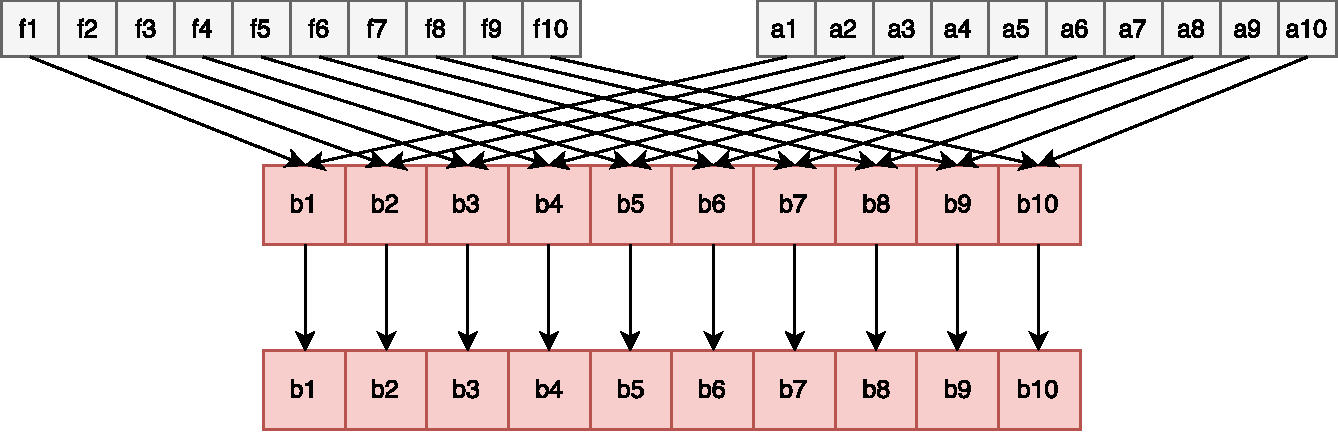
\includegraphics[scale=0.5]{images/parEvalNMulticore}
\end{center} %$ %% formatting

\subsubsection{ParMonad}
The \code{Par} monad\footnote{It can be found in the \texttt{monad-par} package on hackage under \url{https://hackage.haskell.org/package/monad-par-0.3.4.8/}.} introduced by \citet{monad_par_paper_2011}, is a monad designed for composition of parallel programs.


Our parallel evaluation function \code{parEvalN} can be defined by zipping the list of \code{[a -> b]} with the list of inputs \code{[a]} with the application operator \code{\$} just like with Multicore Haskell. Then, we map over this not yet evaluated lazy list of results \code{[b]} with \code{spawnP :: NFData a => a -> Par (IVar a)} to transform them to a list of not yet evaluated forked away computations \code{[Par (IVar b)]}, which we convert to \code{Par [IVar b]} with \code{sequenceA}. We wait for the computations to finish by mapping over the \code{IVar b}'s inside the \code{Par} monad with \code{get}. This results in \code{Par [b]}. We finally execute this process with \code{runPar} to finally get \code{[b]} again.

\textbf{\textcolor{red}{explain problems with laziness here. Problems with torus}}

\begin{lstlisting}[frame=htrbl]
parEvalN :: (NFData b) => [a -> b] -> [a] -> [b]
parEvalN fs as = runPar $ 
	(sequenceA $ map (spawnP) $ zipWith ($) fs as) >>= mapM get
\end{lstlisting}
\begin{center}
	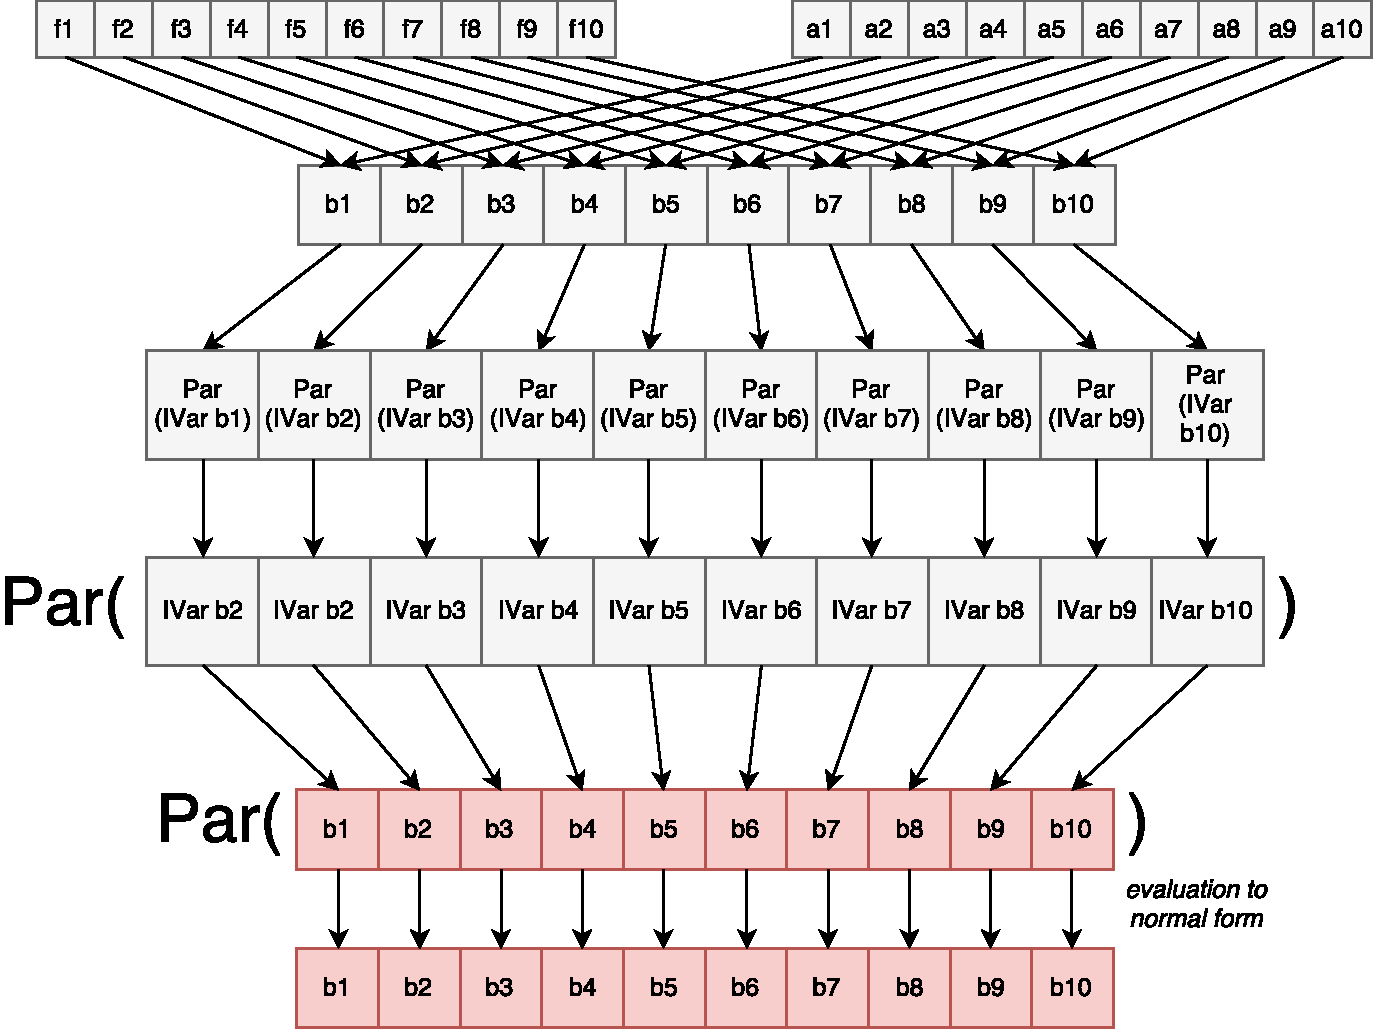
\includegraphics[scale=0.5]{images/parEvalNParMonad}
\end{center}

\subsubsection{Eden}
Eden \cite{eden,Loogen2012} is a parallel Haskell for distributed memory and comes with a MPI and a PVM backends.\footnote{See also \url{http://www.mathematik.uni-marburg.de/~eden/} and \url{https://hackage.haskell.org/package/edenmodules-1.2.0.0/}.} This means that it works on clusters as well so it makes sense to have a Eden-based backend for our new parallel Haskell flavour.

Eden was designed to work on clusters, but with a further simple backend it operates on multicores. However, in contrast to many other parallel Haskells, in Eden each process has its own heap. This seems to be a waste of memory, but with distributed programming paradigm and individual GC per process, Eden yields good performance results also on multicores \cite{arcs-dc,no_pain}.

While Eden also comes with a monad \code{PA} for parallel evaluation, it also ships with a completely functional interface that includes
\\
\code{spawnF :: (Trans a, Trans b) => [a -> b] -> [a] -> [b]}.
\\
This allows us to define \code{parEvalN} directly:

\begin{lstlisting}[frame=htrbl]
parEvalN :: (Trans a, Trans b) => [a -> b] -> [a] -> [b]
parEvalN = spawnF 
\end{lstlisting}
\begin{center}
	\includegraphics[scale=0.5]{images/parEvalNEden}
\end{center}

\paragraph{Eden TraceViewer}
To comprehend the efficiency and the lack thereof in a parallel program, an inspection of its execution is extremely helpful. While some large-scale solutions exist \cite{Geimer2010}, the parallel Haskell community mainly utilises the tools Threadscope \cite{Wheeler2009} and Eden TraceViewer\footnote{See ..... on hackage for the last available version of Eden TraceViewer. There was an effort to implement the TraceViewer using modern web technologies \cite{traceviewer-web}.} \cite{Berthold2007a}. In the next sections we will present some \emph{traces}, the post-mortem process diagrams of Eden processes and their activity.

In a trace, the $x$ axis shows the time, the $y$ axis enumerates the machines and processes. A~trace shows a running process in green, a blocked process is red. If the process is \enquote{runnable}, \ie it may run, but does not, it is yellow. The typical reason for then is GC. An inactive machine where no processes are started yet, or all are already terminated, is shows as a blue bar. A~comminication from one process to another is represented with a black arrow. A~stream of communications, \eg a transmitted list is shows as a dark shading between sender and receiver processes.


%%% Local Variables:
%%% mode: latex
%%% TeX-master: "main"
%%% End:
